% Created 2020-10-25 So 23:03
% Intended LaTeX compiler: pdflatex
\UseRawInputEncoding

\documentclass[11pt]{scrartcl}
\usepackage[utf8]{inputenc}
\usepackage[T1]{fontenc}
\usepackage[ngerman]{babel}
\usepackage{graphicx}
\usepackage{grffile}
\usepackage{longtable}
\usepackage{wrapfig}
\usepackage{rotating}
\usepackage[normalem]{ulem}
\usepackage{amsmath}
\usepackage{trfsigns}
\usepackage{textcomp}
\usepackage{amssymb}
\usepackage{capt-of}
\usepackage{MnSymbol}
\usepackage{mathtools}
\usepackage{setspace}
\usepackage{nicematrix}
\usepackage{varwidth}
\usepackage{pdfpages}
% \usepackage{getlab}
\usepackage{listings}
\usepackage{pdfpages}
\usepackage[straightvoltages, european resistors, american inductors]{circuitikz}
\usetikzlibrary{arrows.meta}
\tikzset{FARROW/.style={arrows={-Triangle[angle=45:2.0mm]}}}


\definecolor{darkspringgreen}{rgb}{0.09, 0.45, 0.27}    % Farbe für die Kommentare bei Listings
\lstset{
  language= Matlab,                     % Setzt die Sprache
  basicstyle=\scriptsize\ttfamily,     % Setzt den Standardstil
  % keywordstyle=\color{red}\bfseries,    % Setzt den Stil für Schlüsselwörter
  identifierstyle=\color{blue},        % Identifier bekommen keine gesonderte formatierung
  commentstyle=\color{darkspringgreen},        % Stil für Kommentare
  stringstyle=\ttfamily,             % Stil für Strings (gekennzeichnet mit "String")
  breaklines=true,             % Zeilen werden umgebrochen
  numbers=left,                 % Zeilennummern links
  numberstyle=\tiny,             % Stil für die Seitennummern
  frame=single,                 % Rahmen
  % backgroundcolor=\color{myGrey},     % Hintergrundfarbe
  % caption={Java-Code},             % Caption
  tabsize=2                % Größe der Tabulatoren
}



\newcommand{\GETHeader}[6]{%
  \begin{titlepage}
    \pagestyle{empty} \enlargethispage*{25cm}\samepage{
      \vspace*{-2.5cm}
      \begin{center}
        %
        \begin{tabular}[b]{lr}
          %
          \hspace*{-1.5cm}
          \begin{tabular}{p{3.8cm}}
            
\includegraphics[width=3.8cm]{./Figures/TUGraz}
          \end{tabular}
          %
          \hspace*{-1cm}
          %
          %
          \begin{tabular}{p{13.8cm}}
            \begin{flushright}
              \large
              Institut für Grundlagen und Theorie der Elektrotechnik\\
              ~\\
            \end{flushright}
          \end{tabular}
        \end{tabular}

        \vspace*{2.2cm}
        %
        \Huge {Elektrische Netzwerke und Mehrtore \\ Übung\\} %
        \vspace*{.5cm} \Large{ Wintersemester 2020\\}
        %
        \vspace*{1.5cm}

        \Huge{\textbf{#1}\\}

        %
        % \vspace*{0.8cm} \Large{Übungsdatum: {#2}\\}
        %
        \vspace*{1cm} \vfill
        %
        \Large{Gruppe: {#2}\\} \vspace*{0.5cm}%


        % \Large{Protokollführer(in): {#3}\\} \vspace*{1cm}

        \Large{Gruppenteilnehmer:\\} \vspace*{.1cm}
        % Name der beteiligten Studierenden
        \Large{#3} \vspace{1cm}
        %
        %
        \Large{Vortragende: #4\\} \vspace*{.1cm}   %\vspace*{1.5cm}
        % \Large{Betreuer(in): #6\\}
        \vspace*{1.5cm}
        %
        \Large{#5, am #6}
      \end{center}}%
    %
    \clearpage
  \end{titlepage}}




\newcommand{\vlaplace}[1][]{\mbox{\setlength{\unitlength}{0.1em}%
    \begin{picture}(10,20)%
      \put(3,2){\circle{4}}%
      \put(3,4){\line(0,1){12}}%
      \put(3,18){\circle*{4}}%
      \put(10,7){#1}
    \end{picture}%
  }%
}%

\newcommand{\vLaplace}[1][]{\mbox{\setlength{\unitlength}{0.1em}%
    \begin{picture}(10,20)%
      \put(3,2){\circle*{4}}%
      \put(3,4){\line(0,1){12}}%
      \put(3,18){\circle{4}}%
      \put(10,7){#1}
    \end{picture}%
  }%
}%














\begin{document}

\GETHeader                                                                              %  Bitte Ausfüllen!!!
% ----------------------------
{Protokoll Übung 3: \\ Schaltvorgang Kondensator}                         %  Übungstitel
% ----------------------------
% {25. Mai 2020}                                                                  %  Übungsdatum
% ----------------------------
{04}                                                                   %  Gruppen-Nr.
% ----------------------------
% {Matthias Fottner}                                                                      % Name des Protokollführers oder der Protokollführerin
% ----------------------------
{
  \begin{center}
    \begin{varwidth}{\textwidth}
    \begin{enumerate}
    \item Matthias Fottner
    \item David Keller
    \item  Moritz Woltron
    \end{enumerate}
    \end{varwidth}
\end{center}
}
% ----------------------------
{Helena Grabner}                                                                     %  Laborleiter(in)
% {Übung 2}                                                               %  Betreuer(in)
% ----------------------------
{Graz}                                                                                  %  Ort der Protokollerstellung
{\today}                                                                %  Datum Protokollerstellung


\newcommand{\unit}[1]{\,\text{#1}}


\tableofcontents

\newpage


\allowdisplaybreaks

\section{Bestimmen des Anfangszustands von $u_C$} % David
\subsection{Schaltplan zur Schalterposition a}

\begin{figure}[!htb]
\begin{center}
        \begin{circuitikz} [european resistors, scale=1]
                \clip (-2,-5.7) rectangle (12.5, 5);

                \draw(0,0) to [R=$R_3$, v={\color{blue}{$U_{R3}$}}, i={\color{red}{$I_{R3}$}}, *-*] (4,0);
                \draw(4,0) to [R=$R_4$, v={\color{blue}{$U_{R4}$}}, i={\color{red}{$I_{R4}$}}] (4,4);
                \draw(4,0) to [R=$R_2$, v<={\color{blue}{$U_{R2}$}}, i<={\color{red}{$I_{R2}$}}] (4,-4);



                \draw(0,0) node[label={[font=\footnotesize]-190:n3}] {} to (0,4);
                \draw(0,4) to[isource, i<={\color{red}{$I_{S2}$}}, -*] (4,4) node[label={[font=\footnotesize]90:n2}] {};
                \draw(4,4) to [R=$R_5$, v={\color{blue}{$U_{R5} = 0\unit{A}$}}, i={\color{red}{$I_{R5} = 0\unit{A}$}}, -o] (8,4);
                \draw(8,4) to (10,4);

                \draw(0,0) to[vsource, v<={\color{blue}{$U_{S1}$}}, i<={\color{red}{$I_{S1}^?$}}] (0,-4);
                \draw(0,-4) to [R=$R_1$, v={\color{blue}{$U_{R1}$}}, i={\color{red}{$I_{R1}$}}, *-*] (4,-4) node[rground]{};
                \draw(4,-4) to [short, -o] (8,-4);
                \draw(8,-4) to (10,-4);
                \draw(10,-4) to [C, v<={\color{blue}{$u_{C} = 0\unit{A}$}}, i<={\color{red}{$i_{C} = 0\unit{A}$}}] (10,4);

                \draw[FARROW, green!50!black] (-0.2, 0) to[bend left=-90, looseness=2.2] node[below left]{$U_{n3}$} (3.9,-4.2);
                \draw[FARROW, green!50!black] (4.1, 3.95) to[bend right=-75, looseness=0.9] node[below right]{$U_{n4}$} (4.4,-3.9);
                \draw[FARROW, green!50!black] (4.1, 0) to[bend right=-75, looseness=0.7] node[below right]{$U_{n1}$} (4.4,-3.7);
                \draw[FARROW, green!50!black] (0.1, -3.8) to[bend right=-75, looseness=0.5] node[above]{$U_{n2}$} (3.9,-3.7);

                %\draw [brown] (current bounding box.south west) rectangle (current bounding box.north east);
                %\draw[gray,step=0.25] (-6,-3) grid (16.5, 11);


        \end{circuitikz}
\end{center}
\caption{Netzwerk mit allen eingezeichneten Strömen, (Knoten-)spannungen und Knoten}
\label{fig:schaltplan_a}
\end{figure}

\pagebreak

\subsection{Erstellen der erweiterten KSV-Matrix}
\begin{align*}
  \renewcommand{\arraystretch}{1.5}
  \begin{bNiceArray}[first-row, first-col]{c:c:c:c:c}
    & n1 & n2 & n3 & n4 & \color{red}{I_{S1}^?} \\
    n1 & G_2+G_3+G_4 & 0 & -G_3 & -G_4 & 0 \\
    \hdottedline
    n2 & 0 & G_1 & 0 & 0 & 1 \\
    \hdottedline
    n3 & -G_3 & 0 & G_3 & 0 & -1 \\
    \hdottedline
    n4 & -G_4 & 0 & 0 & G_4 & 0 \\
    \hdottedline
    \color{red}{I_{S1}^?} & 0 & 1 & -1 & 0 & 0
  \end{bNiceArray}
                                             \begin{Bmatrix}
                                               U_{n1} \\
                                               U_{n2} \\
                                               U_{n3} \\
                                               U_{n4} \\
                                               \color{red}{I_{S1}^?}
                                             \end{Bmatrix} =
  \begin{Bmatrix}
    0 \\
    0 \\
    \color{red}{I_{S2}} \\
    \color{red}{-I_{S2}}\\
    \color{blue}{U_{S1}}
  \end{Bmatrix}\\
\end{align*}



Man erhält mithilfe von Matlab für $x$:
\begin{equation*}
  \renewcommand{\arraystretch}{1.5}
  x = \begin{Bmatrix}
    U_{n1} \\
    U_{n2} \\
    U_{n3} \\
    U_{n4} \\
    I_{S1}^?
  \end{Bmatrix} =
  \begin{Bmatrix}
    -3,36 \unit{V} \\
    2,24 \unit{V} \\
    -7,76 \unit{V} \\
    -4,32 \unit{V} \\
    -0,56 \unit{A}
  \end{Bmatrix}
\end{equation*}

\subsection{Bestimmen von $u_C$} \label{sec:u_c}

Wie sich im Schaltplan in Abbildung \ref{fig:schaltplan_a} erkennen lässt, entspricht $U_{C,a} = U_{n4}$:

\begin{equation*}
  U_{C,a} = U_{n4} = -4,32 \unit{V}
\end{equation*}




\section{Aufstellen der Differentialgleichung} % Matthias
\subsection{Schaltplan zur Schalterposition b}
\begin{circuitikz}
  \clip (-0.8,-1) rectangle (11.5, 4.8);
  \draw (0,0) to[C, v<={\color{blue}{$u_C$}}, i<={\color{red}{$i_C$}}] ++ (0,4)
  to[short, -o] ++ (2,0)
  to[R=$R_5$, v<={\color{blue}{$u_{R5}$}}, i<={\color{red}{$i_{R5}$}}, o-*] ++ (4,0)
  to[R=$R_7$, v={\color{blue}{$U_{R7}$}}, i={\color{red}{$I_{R7}$}}, *-] ++ (4,0)
  to[isource, i={\color{red}{$I_{S3}$}}] ++ (0,-4)
  to[short, -o] ++ (-4, 0)
  to[short, *-o] ++ (-4,0)
  to[short, o-] ++ (-2, 0)
  (6,4) to[R=$R_6$, v={\color{blue}{$u_{R6}$}}, i={\color{red}{$i_{R6}$}}] (6,0)
  (6,0) node[rground]{};

  \draw[european voltages, color=green!50!black] (6.5, 4) to[open, v^=$U_{n1}$] (7,0);
  \draw[FARROW, green!50!black] (10.2, 3.8) to[bend left=80, looseness=1.7] node[below right]{$U_{n3}$} (6.5, -0.3);
  % \draw[gray,step=0.25] (-6,-3) grid (16.5, 11);
  % \draw [brown] (current bounding box.south west) rectangle (current bounding box.north east);
\end{circuitikz}

\begin{circuitikz}
  \draw (0,0) to[C, v<={\color{blue}{$u_C$}}] (0,4)
              to[short, -o] ++ (2,0)
              to[R=$R_{Th}$, v<={\color{blue}{$u_{RTh}$}}, i<={\color{red}{$i_C$}}] ++ (4,0)
              to[vsource, v={\color{blue}{$U_{Th}$}}] ++ (0,-4)
              to[short, -o] ++ (-4, 0)
              to[short] ++ (-2,0);
\end{circuitikz}

\subsection{Erstellen der KSV-Matrix}
\begin{align*}
  \renewcommand{\arraystretch}{1.5}
  \begin{bNiceArray}{c:c}
    G_6 + G_7 & -G_7 \\
    \hdottedline
    -G_7 & G_7
  \end{bNiceArray}
                            \begin{Bmatrix}
                              U_{n1} \\
                              U_{n2} \\
                            \end{Bmatrix} =
  \begin{Bmatrix}
    0 \\
    -I_{S3}
  \end{Bmatrix}
\end{align*}

\subsection{Lösen der Differentialgleichung}
\subsubsection{(Laplace Lösung)}
\setlength{\jot}{12pt}
\begin{align*}
  u_C + u_{RTh} &= U_{Th} \\
  u_C + R_{Th} \cdot i_C &= U_{Th} \\
  u_C + R_{Th} \cdot C \cdot u_C^{\prime} &= U_{Th} \\
  u_C^{\prime} + u_C \left( \frac{1}{R_{Th} \cdot C}\right) &= \frac{U_{Th}}{R_{Th} \cdot C} \\
                &\vLaplace \\
  s \cdot u_C(s) - u_C (0) + \left( \frac{1}{R_{Th} \cdot C} \right) u_C(s) &= \frac{U_{Th}}{R_{Th} \cdot C} \cdot \frac{1}{s} \\
  u_C(s) \left(s + \frac{1}{R_{Th} \cdot C}\right) &= \frac{U_{Th}}{R_{Th} \cdot C} \cdot \frac{1}{s} + u_C(0) \\
  u_C(s) &= \frac{U_{Th}}{R_{Th} \cdot C} \cdot\frac{1}{s \left( s + \frac{1}{R_{Th} \cdot C} \right)} + \frac{u_C(0)}{s + \frac{1}{R_{Th} \cdot C}} \\ \\
  \frac{1}{s\left(s + \frac{1}{R_{Th} \cdot C} \right)} &= \frac{A}{s} + \frac{B}{s + \frac{1}{R_{Th}\cdot C}} \\
  A &= \frac{1}{s + \frac{1}{R_{Th} \cdot C}} \Big|_{s=0} = R_{Th} \cdot C \\
  B &= \frac{1}{s} \Big|_{s=-\frac{1}{R_{Th} \cdot C}} = - R_{Th} \cdot C \\ \\
  u_C(s) &= \frac{U_{Th}}{R_{Th} \cdot C} \left( \frac{R_{Th} \cdot C}{s} - \frac{R_{Th} \cdot C}{s + \frac{1}{R_{Th} \cdot C}}\right) + \frac{u_C(0)}{s + \frac{1}{R_{Th} \cdot C}} \\
                &= U_{Th} \cdot \frac{1}{s} + \left( u_C(0) - U_{Th} \right) \frac{1}{s + \frac{1}{R_{Th} \cdot C}} \\
                &\vlaplace \\
  u_C(t) &= U_{Th} + (u_C(0) - U_{Th}) \cdot e^{-\frac{t}{R_{Th} \cdot C}} \\
\end{align*}

Die Funktion ist um $T_0$ nach rechts verschoben. Deswegen gilt:
\begin{align*}
  u_C(t) = \sigma(t-T_0) \left[ U_{Th} + (u_C(0) - U_{Th}) \cdot e^{-\frac{t-T_0}{R_{Th} \cdot C}} \right]
\end{align*}


\subsubsection{Homogene Lösung}
Die inhomogene Differentialgleichung 1. Ordnung lautet:

\begin{equation*}
  u_C^{\prime} + u_C \cdot \frac{1}{R_{Th} \cdot C} =  \frac{U_{Th}}{R_{Th} \cdot C}
\end{equation*}

Der homogene Anteil lässt sich somit folgendermaßen beschreiben:
\begin{equation*}
  u_{C,h}^{\prime} + u_{C,h} \cdot \frac{1}{R_{Th} \cdot C} = 0
\end{equation*}

Aufgrund des Schaltvorgangs zum  Zeitpunkt $t=T_0$, wird die Gleichung um $T_0$ nach rechts verschoben.
Man setzt an:

\begin{align*}
  u_{C,h} &= K \cdot e^{-\lambda \cdot (t-T_0)} \\
  u_{C,h}^{\prime} &= - \lambda \cdot K \cdot e^{-\lambda \cdot (t-T_0)} \\
  \Longrightarrow -\lambda \cdot K \cdot e^{-\lambda \cdot (t-T_0)} + K \cdot e^{-\lambda \cdot (t-T_0)} \frac{1}{R_{Th}\cdot C} &= 0 \\
  \underbrace{K \cdot e^{-\lambda \cdot (t-T_0)}}_{\neq 0} \left( \frac{1}{R_{Th}\cdot C} - \lambda\right) &= 0 \\
  \frac{1}{R_{Th}\cdot C} &= \lambda \\
  \Longrightarrow u_{C,h} &= K \cdot e^{-\frac{t-T_0}{R_{Th}\cdot C}}
\end{align*}

\subsubsection{Partikuläre Lösung}
Für die partikuläre Lösung kann man $u_{C,p} = A$ ansetzen und erhält:
\begin{align*}
  u_{C,p} &= A \\
  u_{C,p}^{\prime} &= 0 \\
  \Longrightarrow 0 + A \cdot \frac{1}{R_{Th}\cdot C} &= \frac{U_{Th}}{R_{Th}\cdot C} \\
  A &= U_{Th}
\end{align*}

Die Gesamtlösung der Differentialgleichung setzt sich nun aus der homogenen und der partikulären Lösung zusammen:
\begin{equation}\label{eq:diff}
  u_C = u_{C,h} + u_{C,p} = K \cdot e^{-\frac{t-T_0}{R_{Th}\cdot C}} + U_{Th}
\end{equation}

\subsubsection{Anfangswertproblem}
In Kapitel \ref{sec:u_c} wurde bereits der Spannungswert des Kondensators $u_{C,a} = u_C(T_0)$ zum Zeitpunkt $t \leq T_0$ ausgerechnet.
Diesen Anfangswert der stetigen Kondensatorspannung $u_C$ zum Zeitpunkt $T_0$ kann man nun dazu verwenden,
den Wert von K aus der Formel \ref{eq:diff} auszurechnen.
\begin{align*}
  u_C (T_0) &= K \cdot \underbrace{e^{\frac{T_0 - T_0}{R_{Th}\cdot C}}}_{=1} + U_{Th} \\
  \Longrightarrow K &= u_C (T_0) - U_{Th}
\end{align*}

\subsubsection{Gesamtlösung}\label{sec:sol}
Setzt man nun den erhaltenen Wert von $K$ in die Formel \ref{eq:diff} ein, so lautet die gelöste Differentialgleichung:
\begin{equation*}
  u_C = (u_C(T_0) - U_{Th}) \cdot e^{-\frac{t}{R_{Th}\cdot C}} + U_{Th}
\end{equation*}

\section{Vergleich mit allgemeiner Lösungsformel}
Transiente Vorgänge lassen sich verallgemeinert mit folgender Lösungsformel lösen:
\begin{equation*}
  x(t) = x_f + \left[ x_0 - x_f \right] \cdot e^{-\frac{t-t_0}{\tau}}
\end{equation*}

$x_0$ entspricht dem Anfangswert, welcher bei $t=T_0$ den Wert $u_C(T_0) = U_{C,a}$ hat.
$x_f$ entsprich dem Endwert, dieser ist in gegebener Schaltung der Wert von $U_{Th}$, da dieser Spannungswert übrig bleibt,
nachdem sich der Kondensator übrig bleibt.
Setzt man für $x_0$ und $x_f$ die entsprechenden Werte in die allgemeine Lösungsformel ein,
so ist diese Form identisch mit der Gesamtlösung aus Kapitel \ref{sec:sol}.


\newpage
\section{Simulation in PSpice}
\subsection{Schalterposition a}
In der Schalterposition a muss der Kondensator $C$ nicht aufgezeichnet werden, da er nach langer Zeit wie ein Leerlauf fungiert.

\begin{center}
  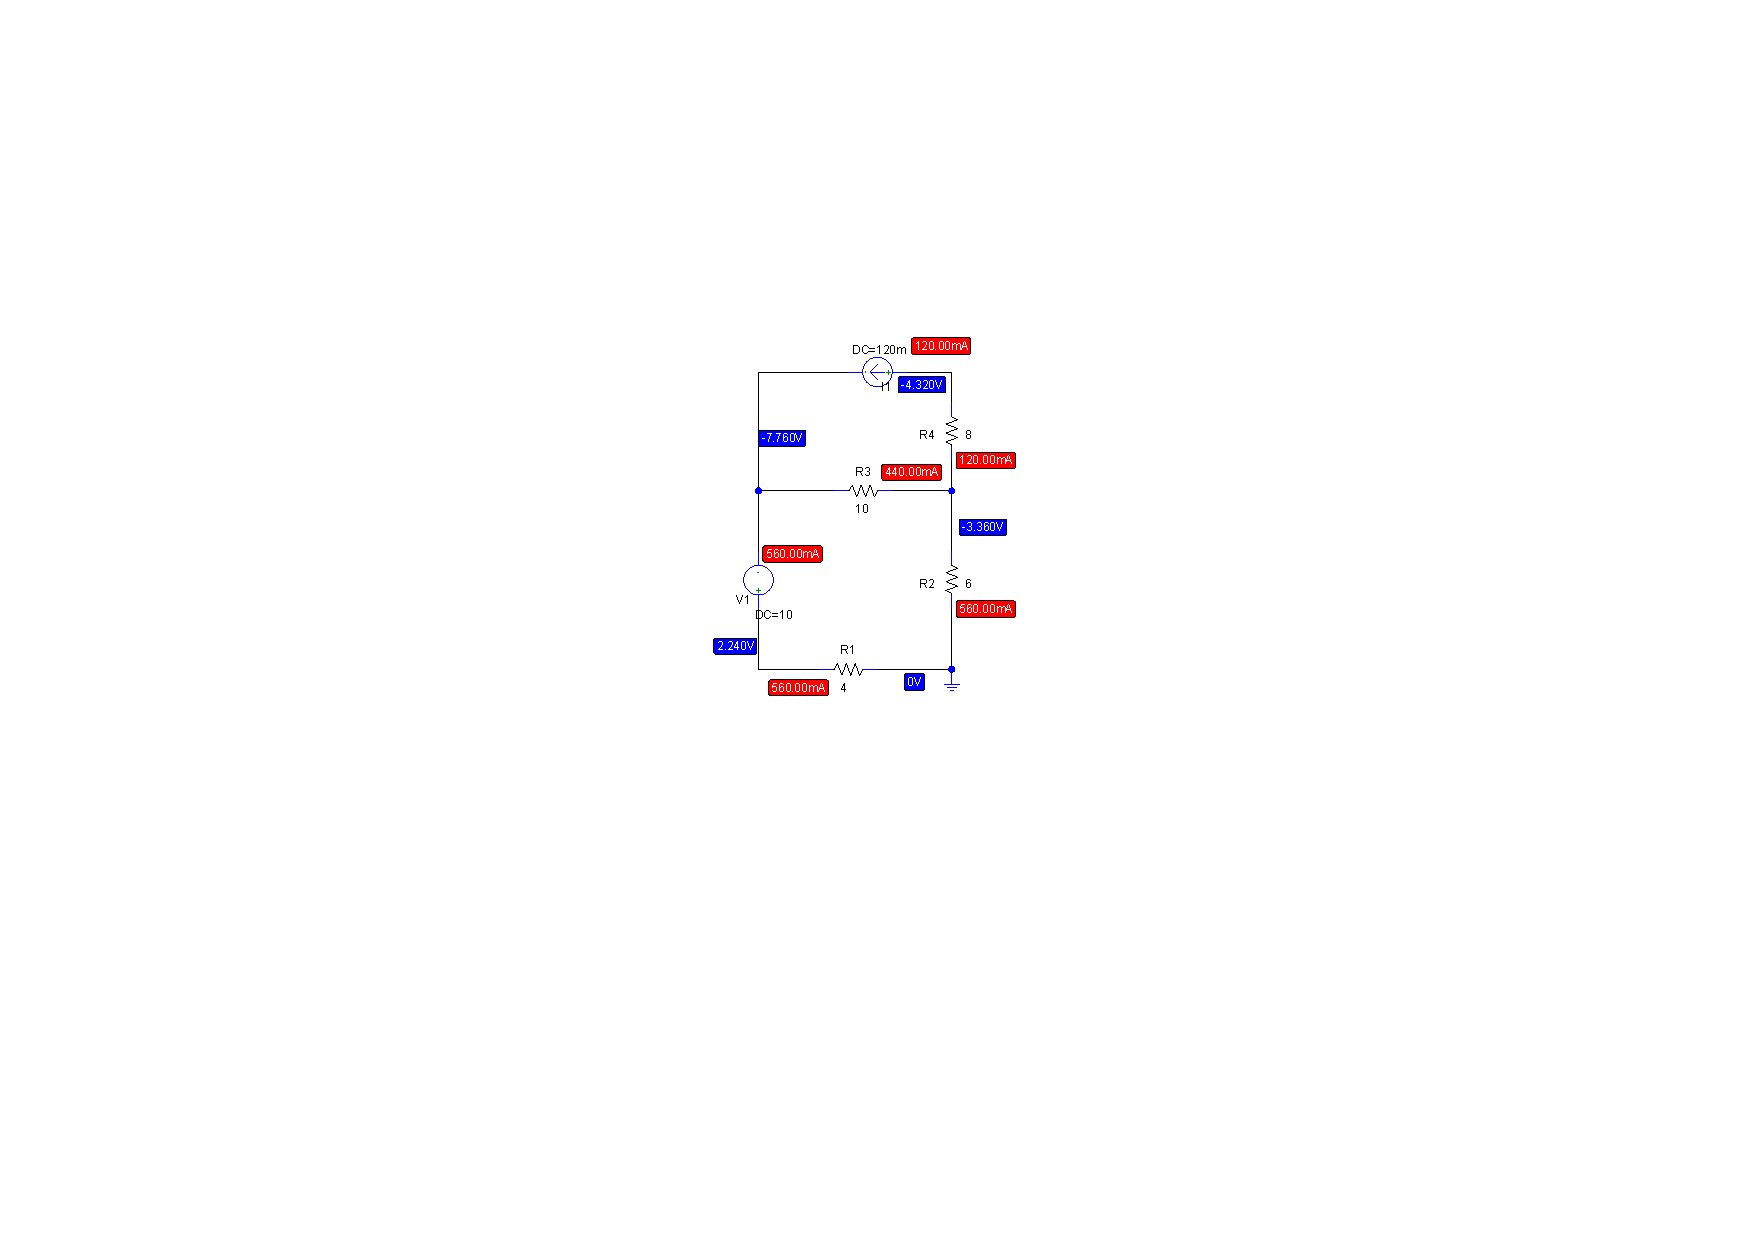
\includegraphics[scale=1.6]{./Assets/SP_a}
  \captionof{figure}{PSpice-Simulation der Schalterposition a}
  \label{fig:a}
\end{center}
\newpage

\subsection{Schalterposition b}
\begin{center}
  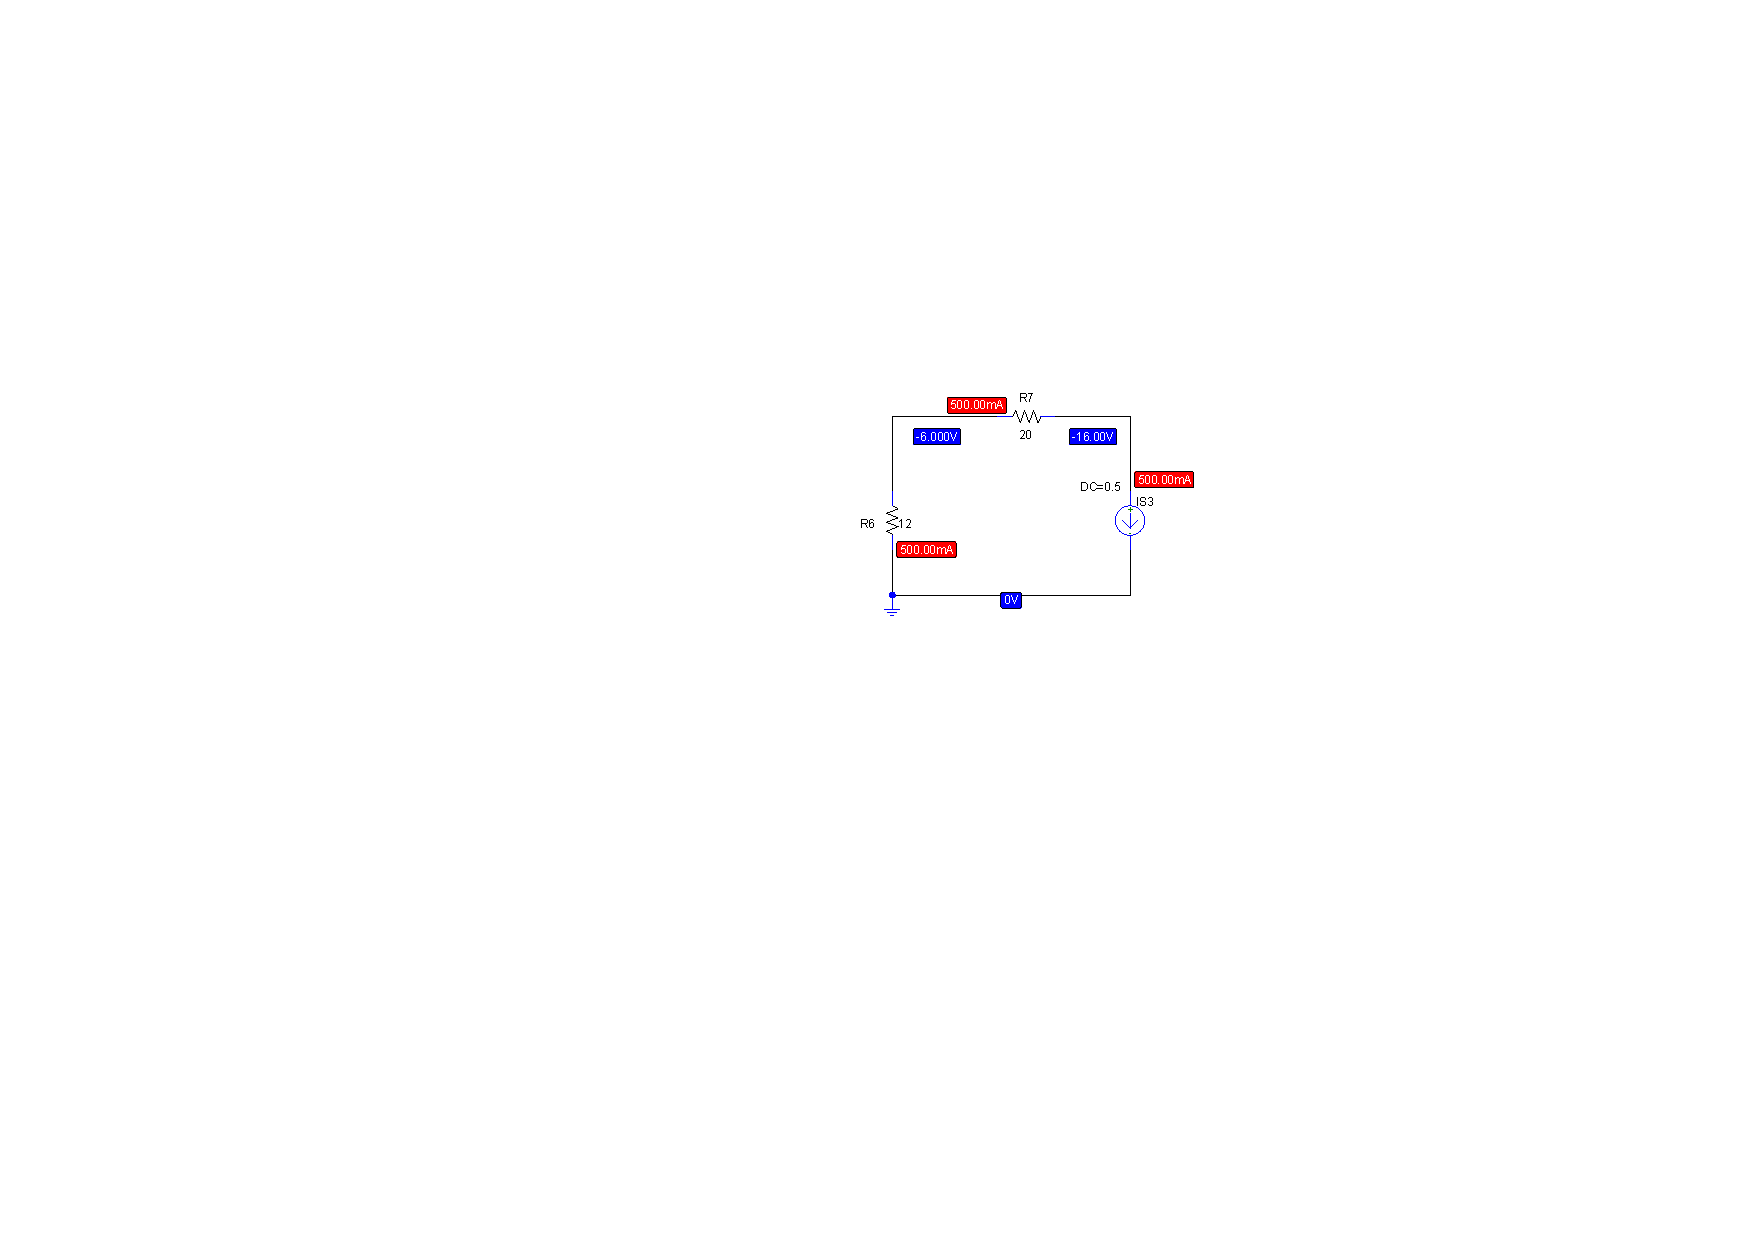
\includegraphics[scale=1.6]{./Assets/SP_b}
  \captionof{figure}{PSpice-Simulation der Schalterposition b}
  \label{fig:b}
\end{center}

\newpage
\subsection{Simulation des Umschaltvorgangs}
In Abbildung \ref{fig:umschalt} ist der Schaltungsaufbau für die Simulation des Umschaltvorgangs zu sehen.
Dabei ist der Schalter tOpen zum Zeitpunkt $0 < t \leq 100 \unit{ms}$ geschlossen, während tClose geschlossen ist.
Zum Zeitpunkt $t > 100 \unit{ms}$ ist tOpen offen und tClose geschlossen.

\begin{center}
  % 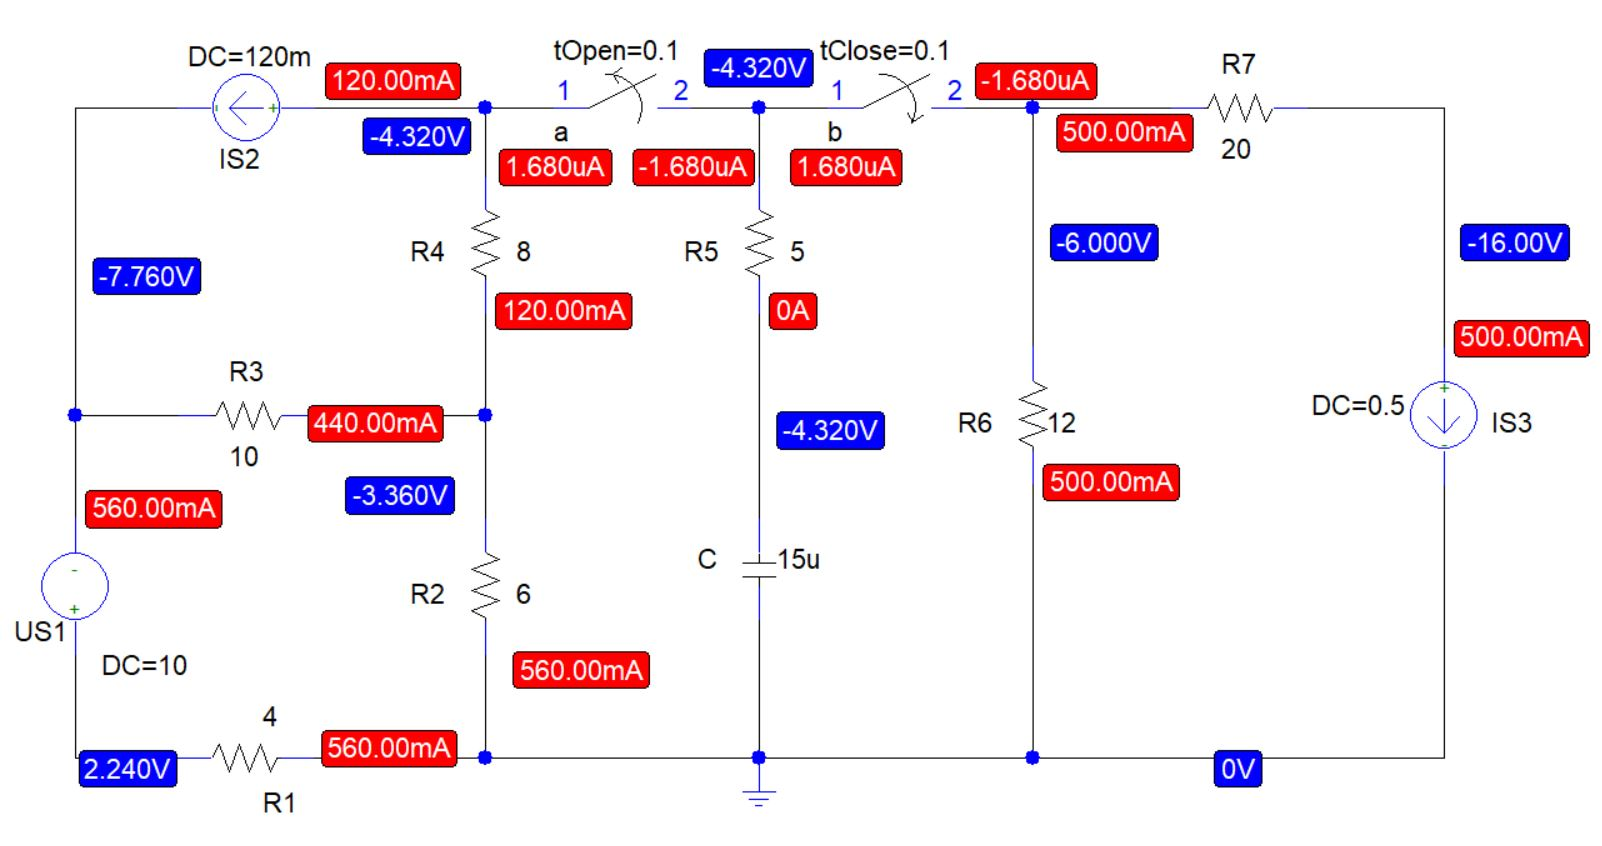
\includegraphics[width=1\linewidth]{./Assets/gesamter Schaltvorgang - PSpice}
  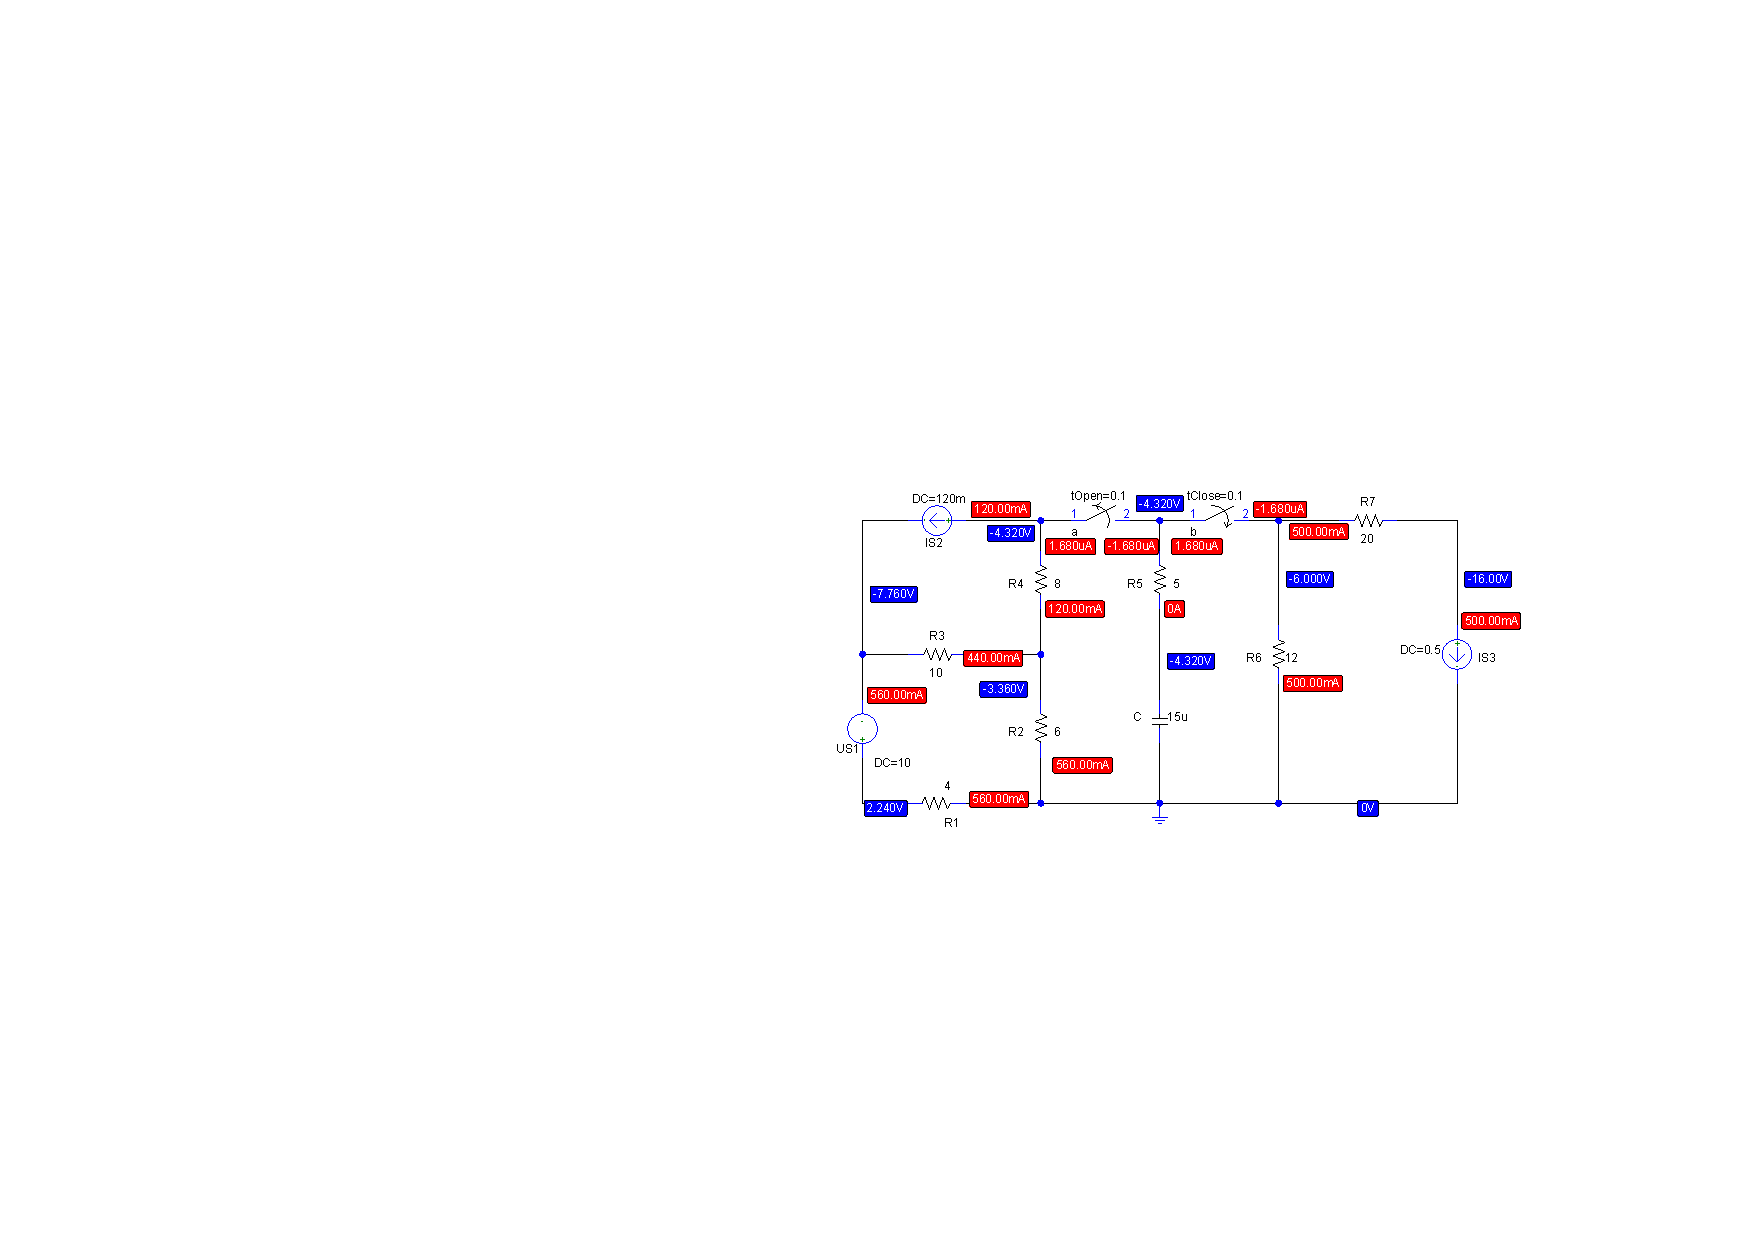
\includegraphics[scale=1.3]{./Assets/gesamter Schaltvorgang.pdf}
  \captionof{figure}{PSpice-Simulation des Umschaltvorgangs}
  \label{fig:umschalt}
\end{center}

\newpage
\section{Matlab-Simulation}
\subsection{Skript}
\lstinputlisting[language=Matlab]{./../Matlab/GR04_UE_03.m}

\subsection{Konsolenoutput}
\begin{lstlisting}[language=Matlab, escapeinside={(*}{*)}]
  U_C_a =

  "-4.3200 V"


  U_Th =

  "-6.0000 V"


  R_Th =

  "17 (*$\Omega$*)"
\end{lstlisting}

\subsection{Plot}
\begin{center}
  % 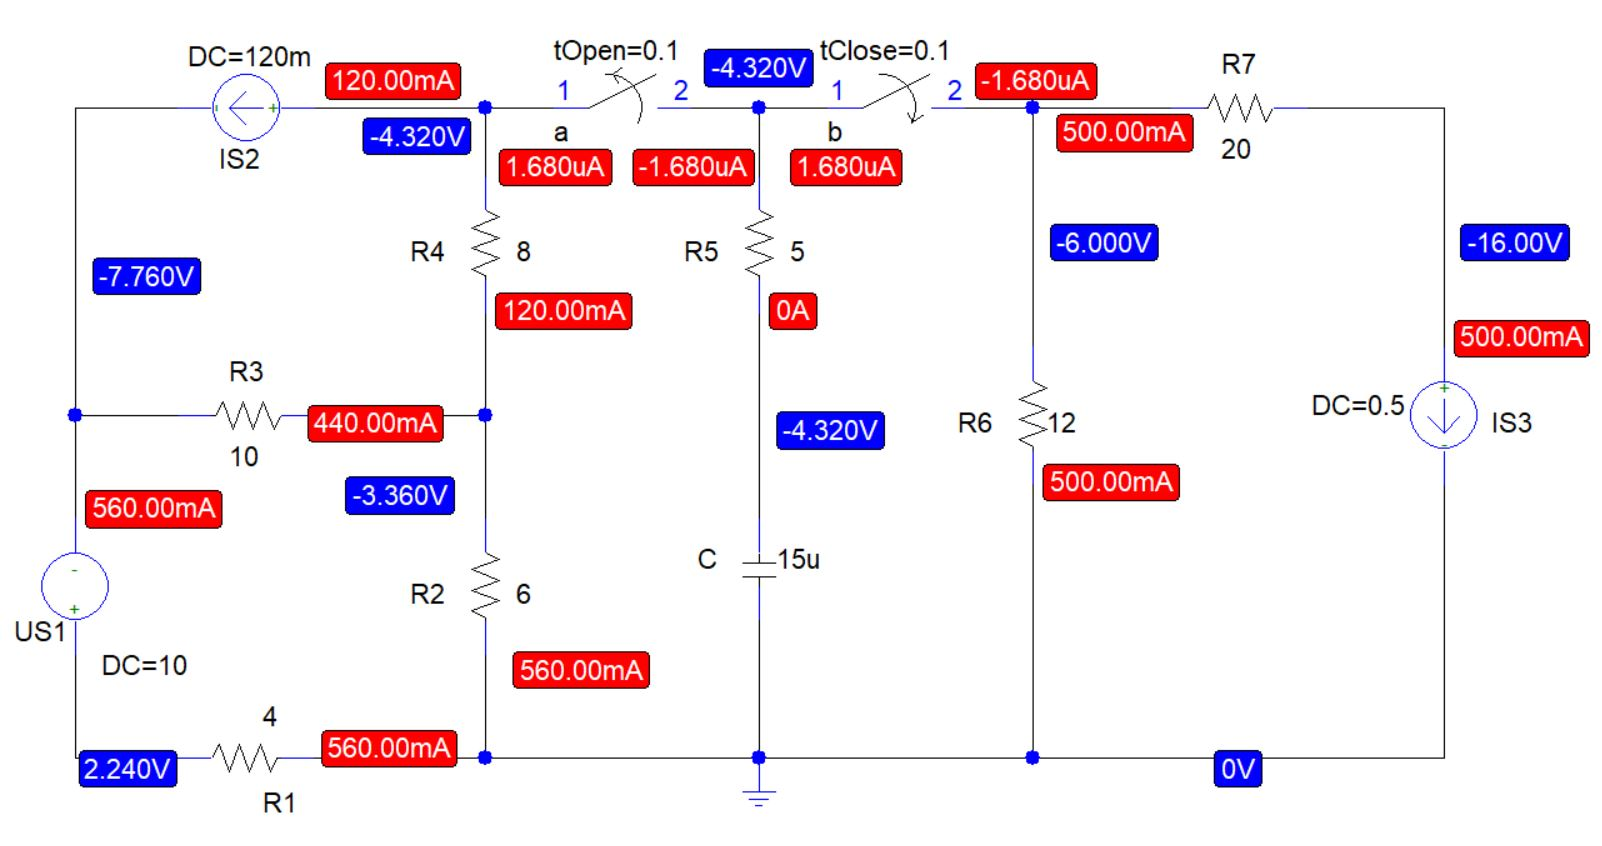
\includegraphics[width=1\linewidth]{./Assets/gesamter Schaltvorgang - PSpice}
  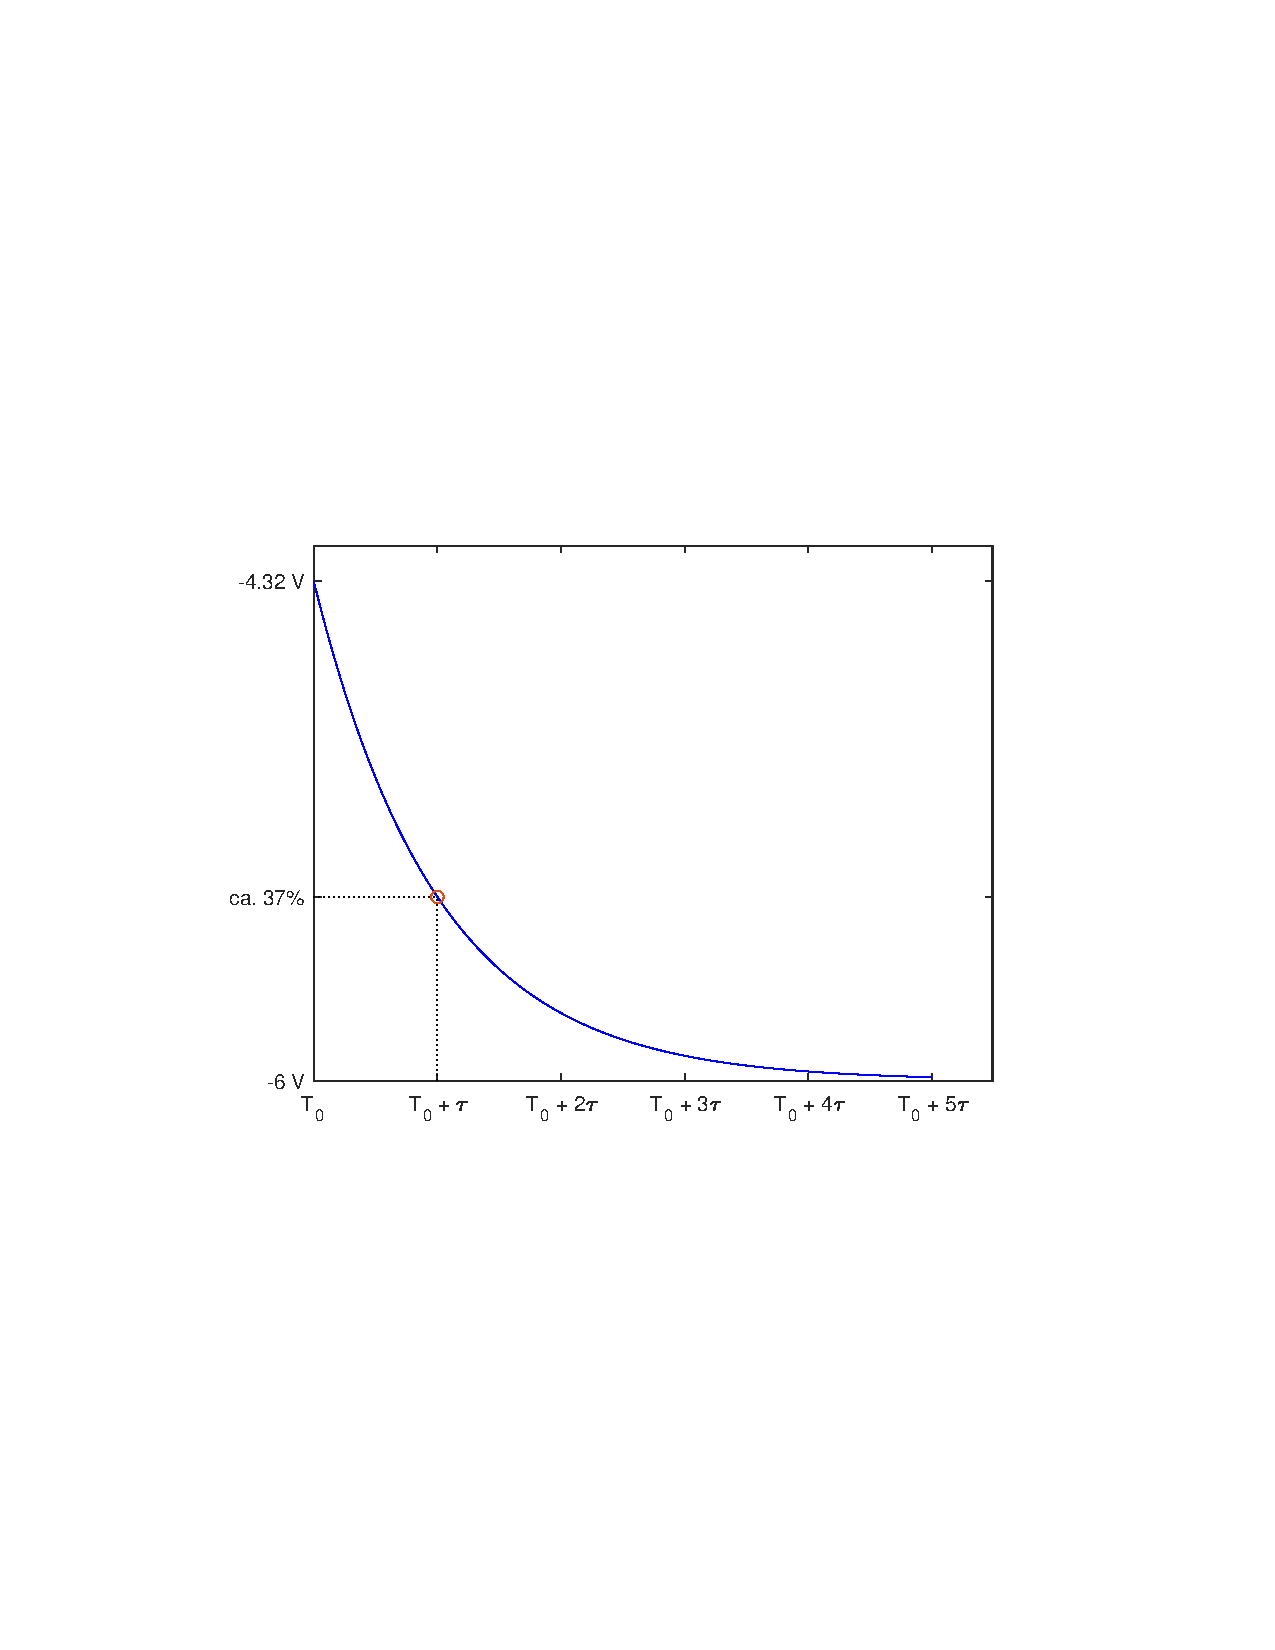
\includegraphics[scale=1]{./Assets/u_C_plot.pdf}
  \captionof{figure}{Matlab Plot des Umschaltvorgangs von $t=T_0$ bis $t=T_0 + 5 \cdot  \tau$}
  \label{fig:umschalt}
\end{center}


\end{document}